% =====================================================================
%  Panel captions --- UC Davis CASMI catalogue
%
%  Every number below is read from catalogue/casmi/panel_data.json as
%  regenerated on the corrected pipeline, and matches the rendered PNG.
%  Macros assumed from the manuscript preamble:
%      \con    intensity-weighted contact  \kappa
%      \Dmass  the mass determination      \mathcal{D}_m
%      \Dcon   the contact determination   \mathcal{D}_c
%  If this file is compiled standalone, define them first.
% =====================================================================

\begin{figure*}[!htbp]
    \centering
    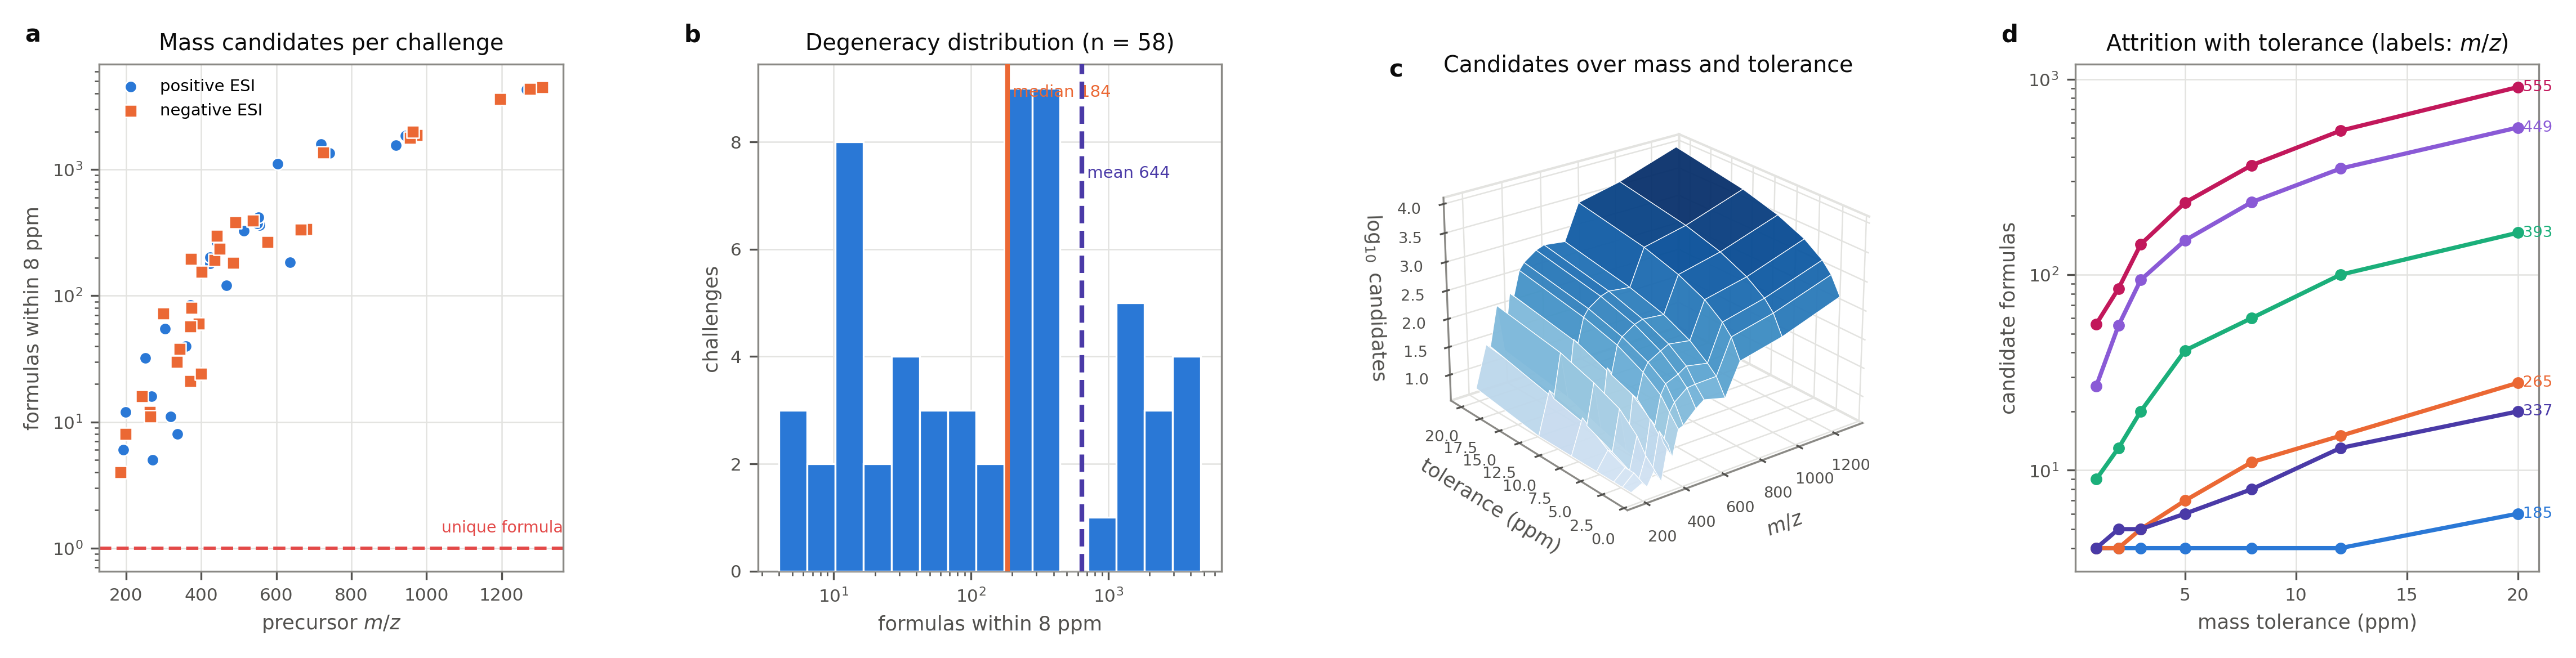
\includegraphics[width=\textwidth]{figures/panel1_degeneracy.png}
    \caption{\textbf{Exact Mass Does Not Determine Formula: The Degeneracy of the Mass Determination.}
    (\textbf{A})~Uncapped count of distinct CHNOPS formulas satisfying the 8~ppm precursor window, plotted against precursor $m/z$ for all 58 challenges and separated by polarity (positive ESI blue, negative ESI orange). The count rises from 4 at the low-mass end to 4500 near $m/z$~1300. The dashed line at a unique formula is the singleton level: no challenge reaches it, so the mass determination $\Dmass$ never resolves to one answer anywhere in this set.
    (\textbf{B})~Distribution of the same 58 counts on a logarithmic axis, median 183 (solid) and mean 644 (dashed). The distribution is strongly right-skewed---half the challenges admit fewer than 183 formulas while the tail extends past 3000---and the bin at $|\Dmass| = 1$ is empty.
    (\textbf{C})~Three-dimensional surface of $\log_{10}$ candidate count over precursor $m/z$ ($185$--$1300$) and mass tolerance ($1$--$20$~ppm) for the 15 challenges carried through the tolerance grid. The surface rises steeply with mass and only gently with tolerance: tightening the window an order of magnitude below the instrument's achievable accuracy does not collapse the count to unity at any mass above the low-mass end. Degeneracy is a property of formula space, not of measurement precision.
    (\textbf{D})~Candidate count against tolerance for six challenges spanning the mass range, each labelled with its precursor $m/z$, on a logarithmic count axis. Attrition is approximately linear in tolerance while the offset between curves is superlinear in mass: challenge 33 ($m/z$~185) holds 4 candidates from 1 to 12~ppm and reaches only 6 at 20~ppm, whereas the $m/z$~555 challenge runs from 56 to 911 over the same sweep. No accessible tolerance isolates a single formula for the heavier precursors.}
    \label{fig:panel1}
\end{figure*}

\begin{figure*}[!htbp]
    \centering
    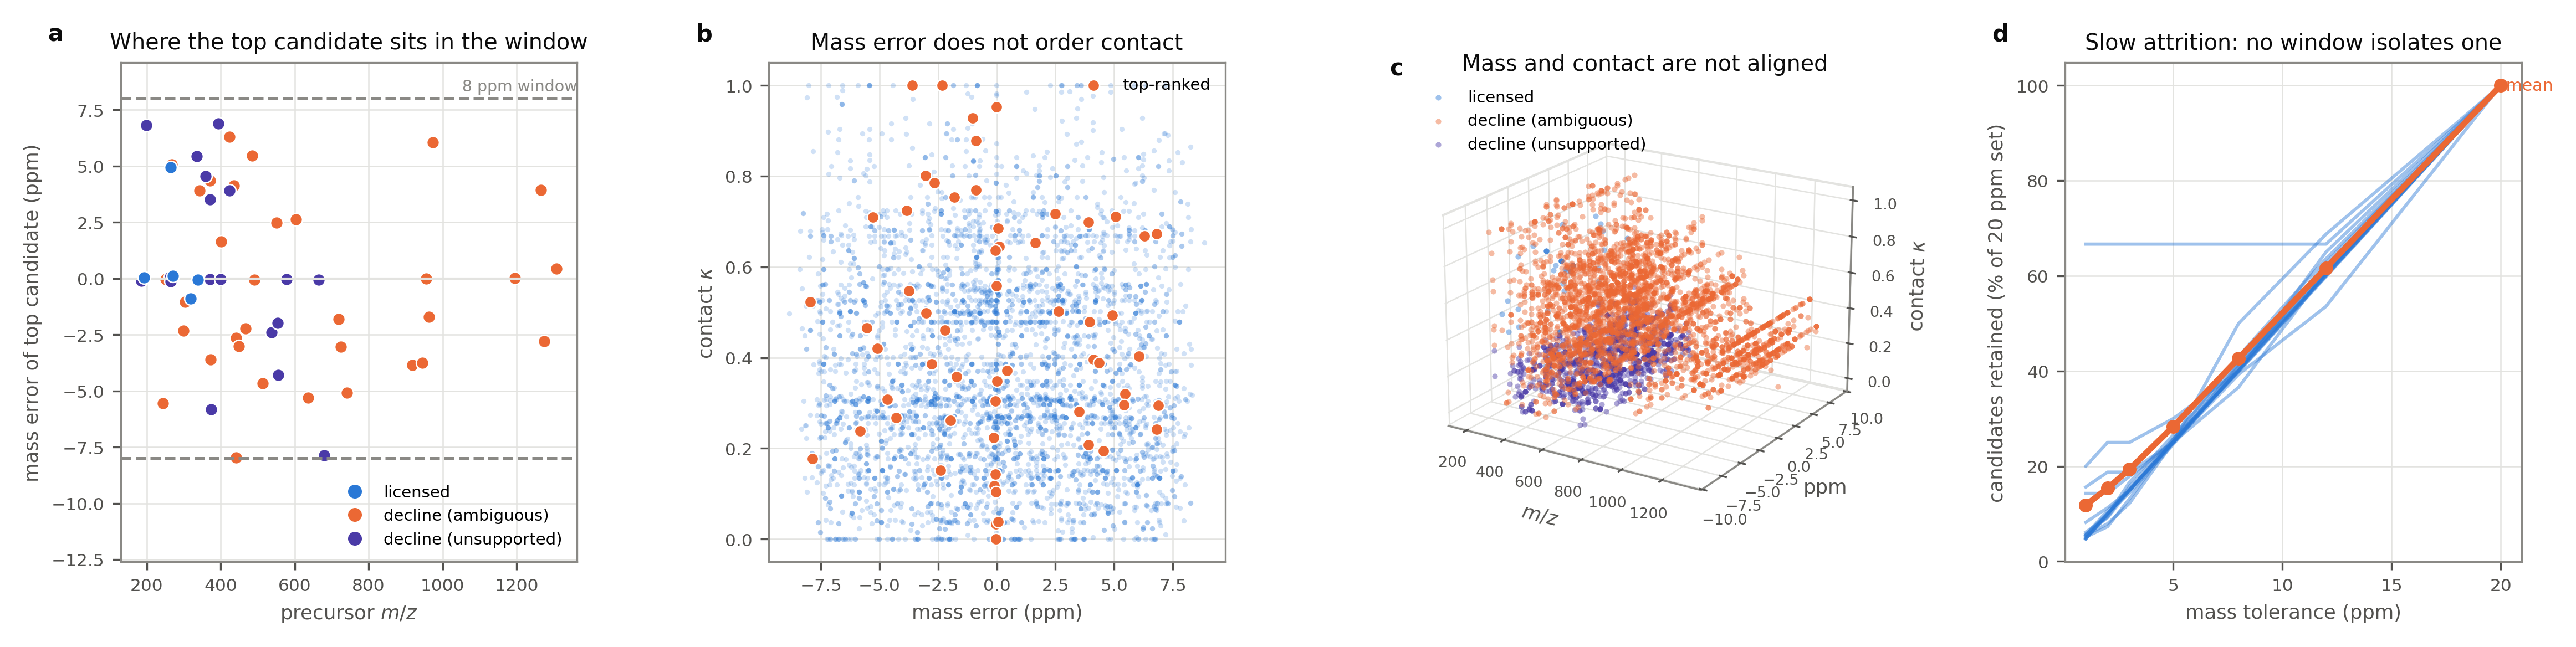
\includegraphics[width=\textwidth]{figures/panel2_tolerance.png}
    \caption{\textbf{Mass Error, Contact, and the Geometry of the 8~ppm Window.}
    (\textbf{A})~Measured precursor mass error of the top-ranked candidate for each challenge against precursor $m/z$, coloured by verdict, with the $\pm 8$~ppm acceptance envelope drawn. Licensed challenges (blue) cluster tightly at zero error---four of the five lie within $\pm 1$~ppm---while the fifth sits at $+4.94$~ppm, well inside the envelope but visibly off-centre. Declining challenges occupy the full width of the window, so position within the envelope does not by itself predict whether an answer will be licensed.
    (\textbf{B})~Contact $\con$ against mass error for all 4684 scored candidates (pale), with the 58 top-ranked candidates overlaid (orange). Contact spans its entire range at every mass error, including at zero: candidates whose mass matches the precursor essentially perfectly take contact values from 0 to 1. Mass error carries no ordering information about contact, which is the empirical content of the claim that $\Dmass$ and $\Dcon$ are independent determinations.
    (\textbf{C})~Three-dimensional scatter of precursor $m/z$, mass error, and contact for every scored candidate, coloured by verdict class. The cloud fills the contact axis at every $(m/z, \text{ppm})$ position rather than forming a ridge or a sheet. This is the geometric form of (B): the two determinations are not aligned, so neither can be recovered from the other.
    (\textbf{D})~Candidates retained as a percentage of the 20~ppm set as the tolerance is tightened, one curve per challenge, with the mean in orange. Retention falls smoothly and slowly---the mean still holds roughly 12\% of the 20~ppm set at 1~ppm, and no curve reaches the single-candidate level. The one stepped curve is challenge 33, the least degenerate in the set, whose retention quantises because it holds only 4 candidates across most of the range. Tightening the window is attrition, not resolution, and this is what motivates a second determination rather than a better first one.}
    \label{fig:panel2}
\end{figure*}

\begin{figure*}[!htbp]
    \centering
    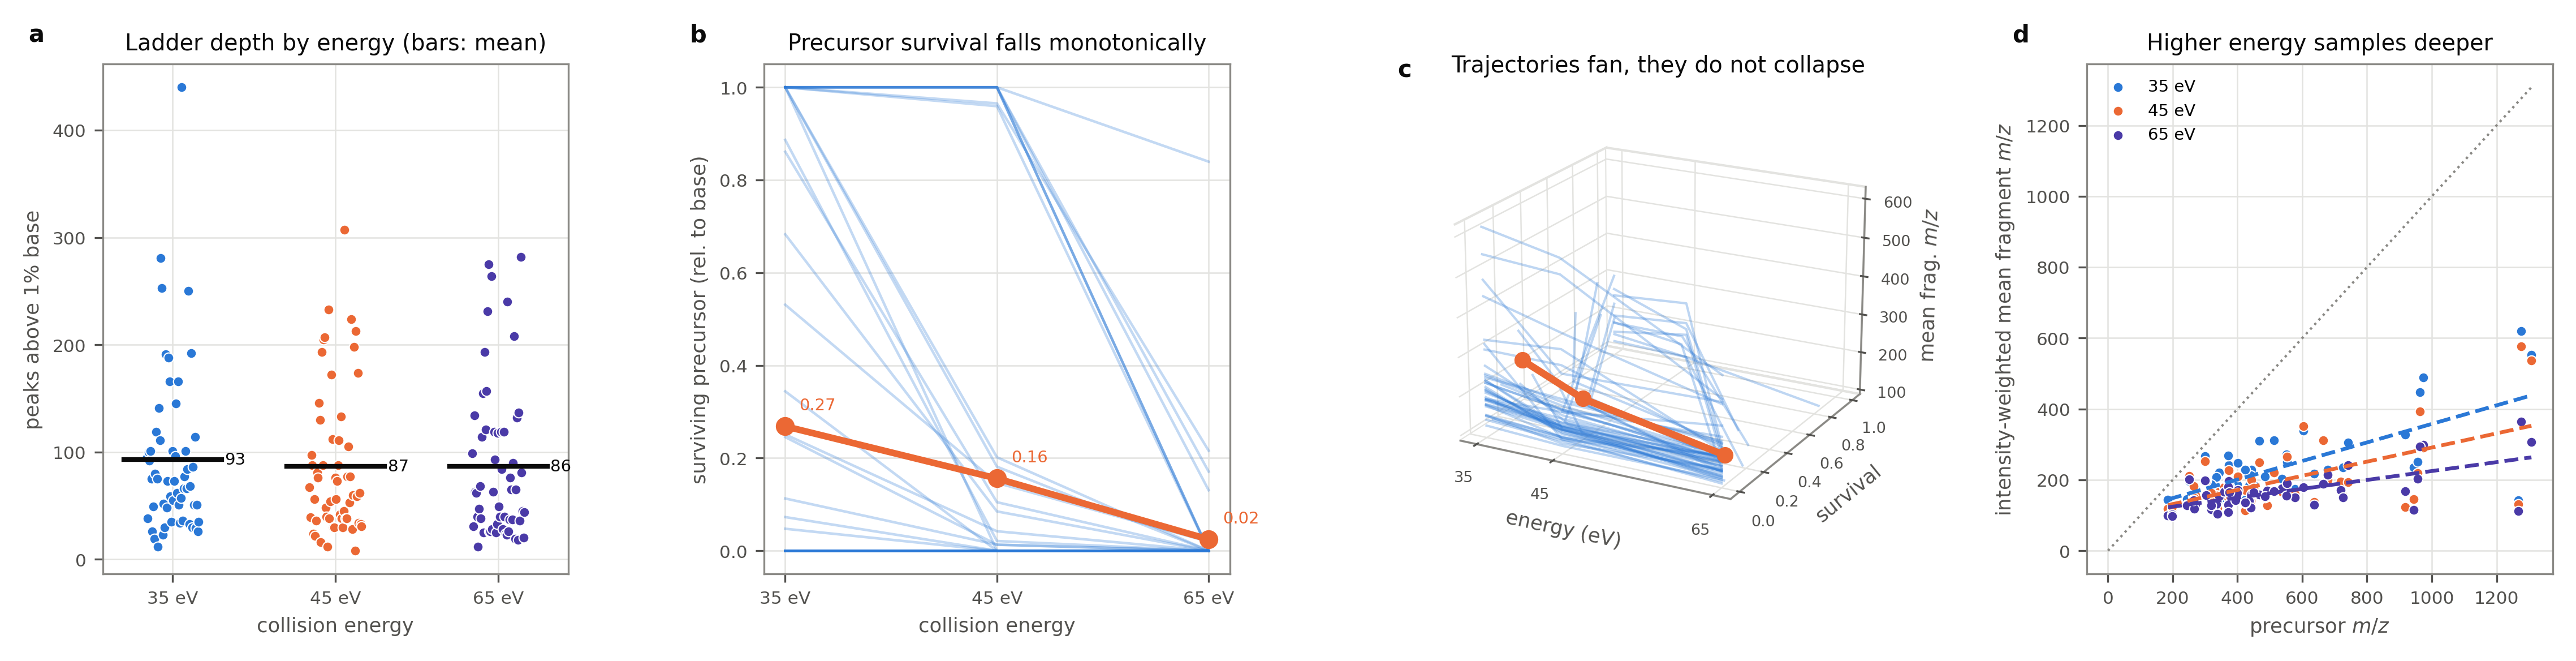
\includegraphics[width=\textwidth]{figures/panel3_energy.png}
    \caption{\textbf{The Three Collision Energies Are Not Redundant.}
    (\textbf{A})~Peak count above 1\% of base peak for each challenge at 35, 45 and 65~eV, with class means marked. The mean ladder depth falls from 93 to 87 to 86 peaks, but the decline is slight relative to the spread and the per-challenge orderings differ: some challenges lose peaks steadily with energy while others gain them at 65~eV, reaching above 280. The three energies are not three samples of one ladder.
    (\textbf{B})~Surviving precursor intensity relative to base peak at each energy, paired by challenge. Survival falls monotonically and steeply across the set, from a mean of 0.27 at 35~eV through 0.16 at 45~eV to 0.02 at 65~eV. By 65~eV the precursor is essentially consumed, so the highest energy contributes fragment structure but almost no surviving parent signal.
    (\textbf{C})~Three-dimensional trajectory of each challenge through collision energy, precursor survival, and intensity-weighted mean fragment $m/z$, with the set mean in orange. The trajectories fan apart rather than collapsing onto the mean: challenges at equal survival reach different fragment masses, and challenges at equal fragment mass differ in survival. Averaging the three energies into one spectrum would discard exactly this spread, which is why the method holds them as separate evidence channels weighted by $w = \mathrm{rel} \times (1 + 0.5(n_{\mathrm{CE}} - 1))$.
    (\textbf{D})~Intensity-weighted mean fragment $m/z$ against precursor $m/z$ at each energy, with fitted lines and the identity diagonal. All three lines lie well below the diagonal and their slopes decrease with energy ($35 > 45 > 65$~eV), so higher energy samples deeper into the fragmentation cascade at every precursor mass. The separation between the fitted lines widens with precursor mass, meaning the three channels become more informative relative to one another precisely where the mass determination is most degenerate.}
    \label{fig:panel3}
\end{figure*}

\begin{figure*}[!htbp]
    \centering
    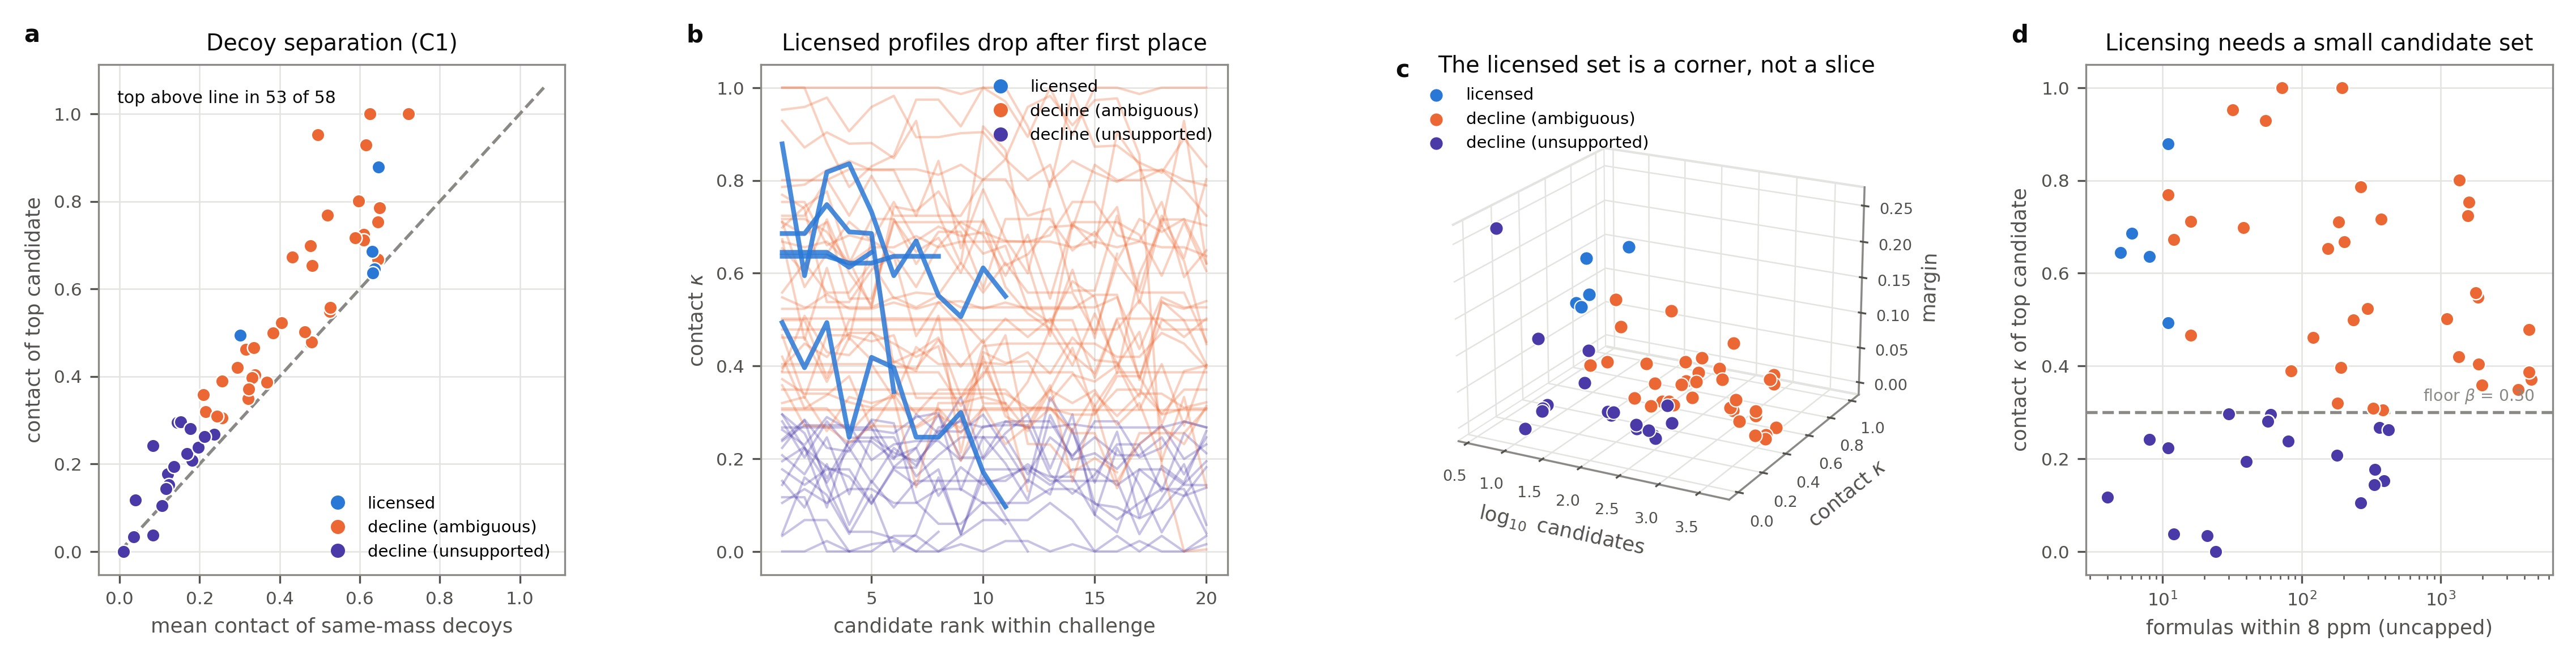
\includegraphics[width=\textwidth]{figures/panel4_contact.png}
    \caption{\textbf{Contact Separates Candidates That Mass Cannot (Control C1).}
    (\textbf{A})~Contact of the top-ranked candidate against the mean contact of its same-mass decoys---every distinct rival formula in the 8~ppm window, de-duplicated, a median of 119 rivals per challenge---one point per challenge, with the line of equality. The top candidate lies above the line in 53 of 58 challenges; mean top contact 0.4689 against mean decoy contact 0.3633, a separation of $+0.1055$. The five points below the line are challenges where the mass-ranked leader is not the best-explaining candidate, and all five decline.
    (\textbf{B})~Ordered contact profile of the twenty highest-scoring candidates within each challenge, one curve per challenge. Licensed cases (blue) fall sharply after first place; ambiguous cases (orange) descend gradually, several remaining near the leader's value through fifth place and beyond. The distinction the method acts on is the shape of this descent, not the height of its first point---an ambiguous challenge can have a higher leading contact than a licensed one.
    (\textbf{C})~Three-dimensional scatter of $\log_{10}$ mass degeneracy, contact, and margin for all 58 challenges, coloured by verdict. The licensed points occupy a corner---low degeneracy, high contact, high margin---rather than a slab cut perpendicular to any single axis. No one of the three coordinates separates the licensed set on its own.
    (\textbf{D})~Contact of the top candidate against uncapped mass degeneracy. The licensed challenges all sit at low degeneracy (5 to 11 candidates), while challenges with several hundred candidates reach high contact without ever licensing. High contact is necessary but not sufficient: it must be high \emph{and} the field it beat must have been thin enough for the margin to be meaningful.}
    \label{fig:panel4}
\end{figure*}

\begin{figure*}[!htbp]
    \centering
    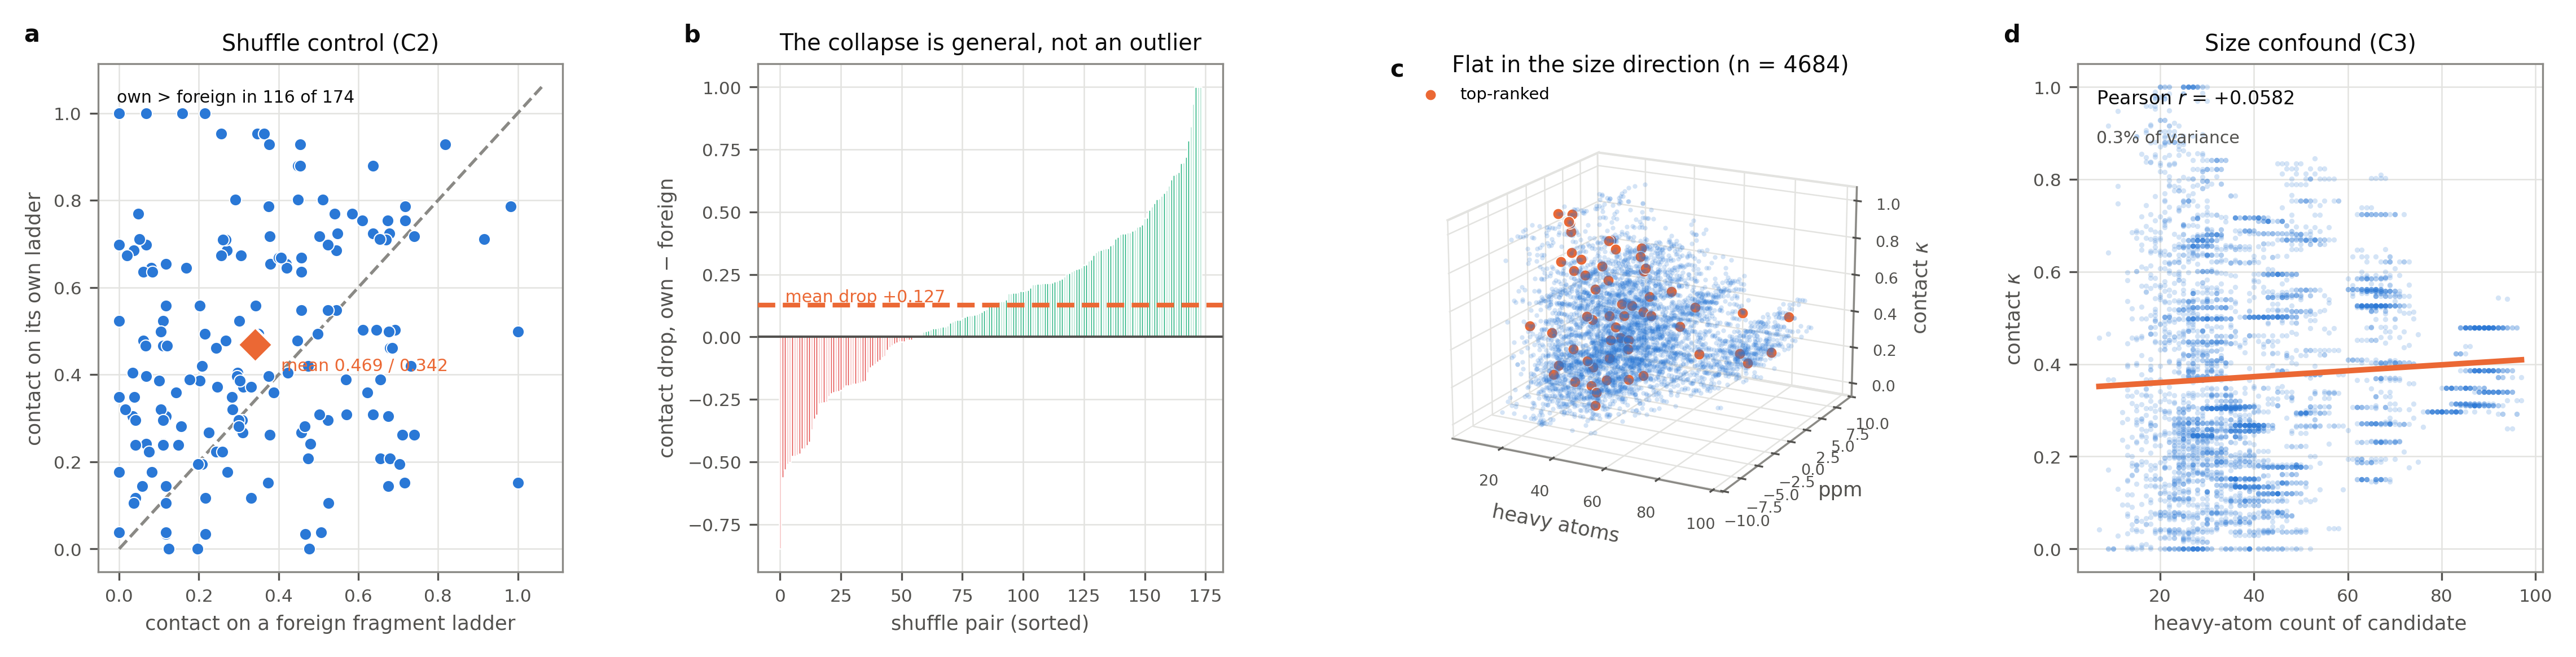
\includegraphics[width=\textwidth]{figures/panel5_controls.png}
    \caption{\textbf{Contact Is Structural: It Is Not Size and It Is Not Coincidence (Controls C2 and C3).}
    (\textbf{A})~Shuffle control. Contact of each top candidate scored on its own fragment ladder against its contact on a foreign ladder drawn from a different challenge of the same polarity---174 pairs, three per challenge, with the set mean as the orange diamond and the line of equality dashed. The mean falls from 0.469 to 0.342. Pairs are formed by filtering to matching polarity \emph{before} drawing rather than by rejection sampling; the biased alternative discards more than half the challenges and inflates this separation roughly twofold.
    (\textbf{B})~Paired contact drop per shuffle pair, sorted, with the mean at $+0.127$. The drop is positive in 116 of 174 pairs and negative in the remaining 58. The effect is therefore carried by a two-thirds majority---general rather than driven by a handful of outliers, but well short of universal. A formula that explains its own ladder usually explains an arbitrary one less well, and sometimes does not.
    (\textbf{C})~Three-dimensional scatter of heavy-atom count, mass error, and contact over all 4684 scored candidate--fragment evaluations, with top-ranked candidates highlighted. The cloud is visibly flat in the size direction across the full range of 7 to 97 heavy atoms: large candidates do not accumulate contact by having more subformulas available to match.
    (\textbf{D})~Contact against heavy-atom count with the fitted line, the two-dimensional form of the C3 correlation. Pearson $r = +0.0582$, so candidate size explains 0.3\% of the variance in contact. The fitted line rises by less than 0.1 in $\con$ across a fourteen-fold range in size, against a licensing floor of 0.30 and a licensing margin of 0.10.}
    \label{fig:panel5}
\end{figure*}

\begin{figure*}[!htbp]
    \centering
    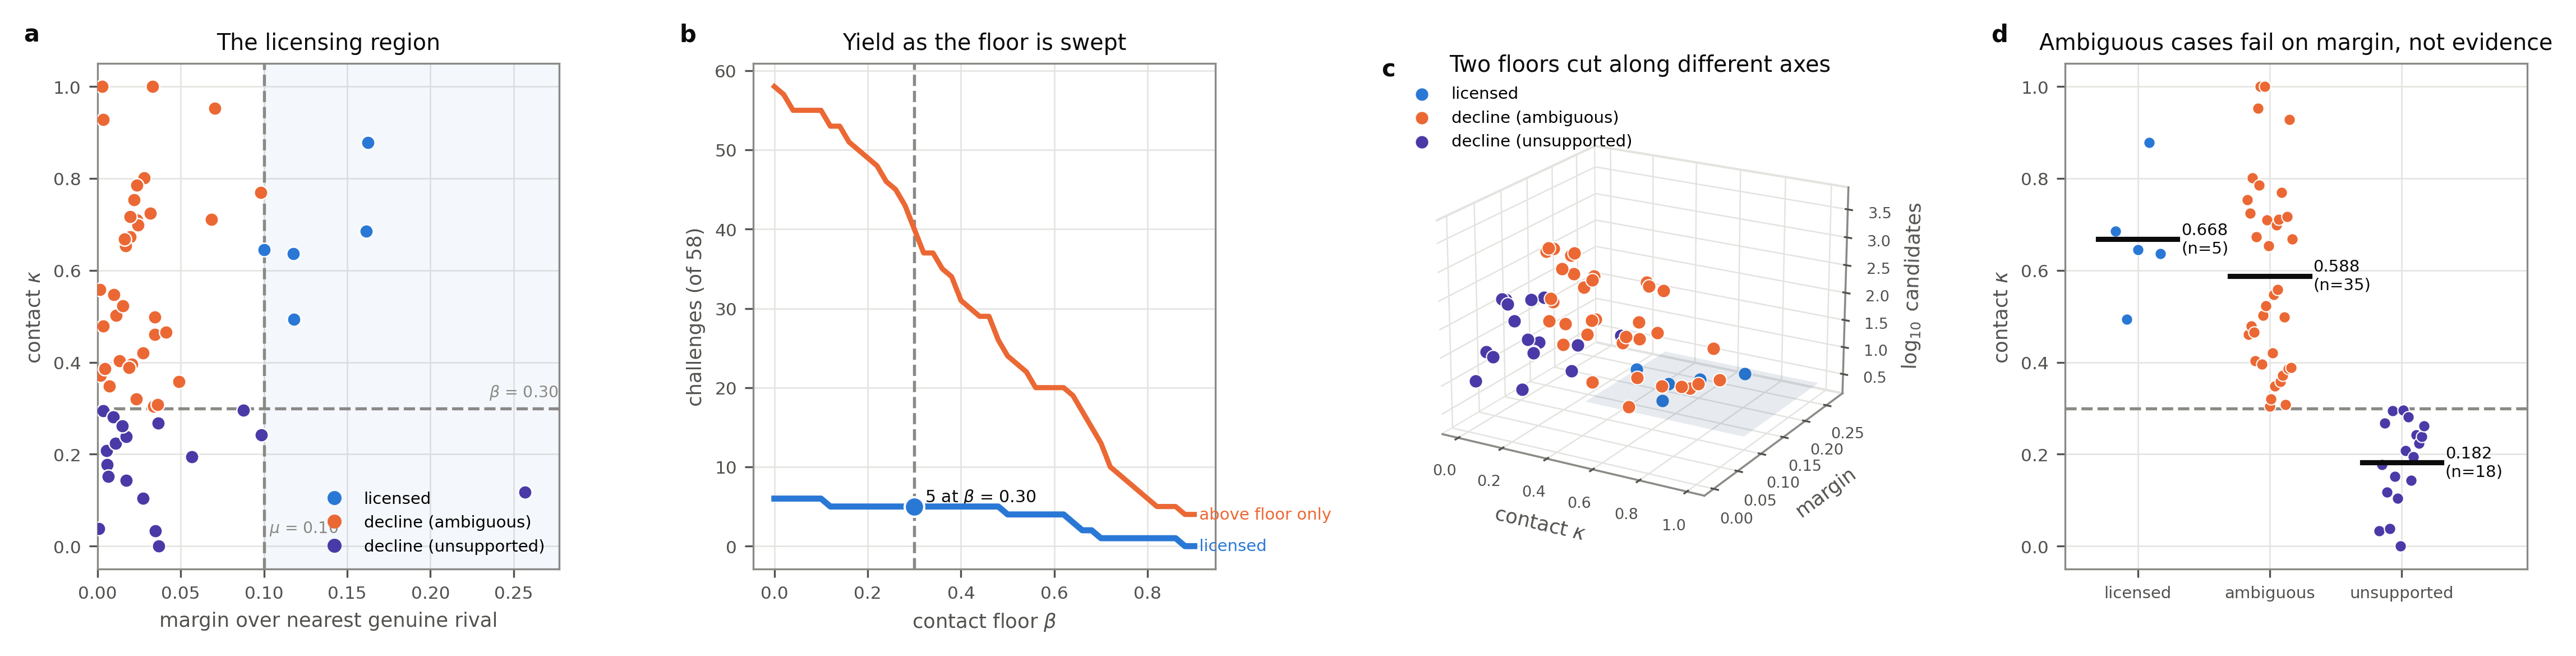
\includegraphics[width=\textwidth]{figures/panel6_licensing.png}
    \caption{\textbf{The Floor, the Decline, and What Declining Buys.}
    (\textbf{A})~Contact against margin over the nearest genuine rival for all 58 challenges, with the licensing region $\con \ge 0.30$ and margin $\ge 0.10$ marked. Five challenges fall inside it. The population immediately outside is dense along the margin axis and sparse along the contact axis, which already shows which of the two floors is doing the work.
    (\textbf{B})~Licensed count and above-floor count as the contact floor $\beta$ is swept from 0 to 0.90, with the chosen $\beta = 0.30$ marked. The two curves separate sharply: the above-floor population falls from 40 challenges at $\beta = 0.30$ to 31 at 0.40 and 24 at 0.50, while the licensed count stays flat at five until $\beta = 0.50$, where it drops to four. Every licensed answer has $\con \ge 0.493$, so the floor can be raised by a third without changing a single verdict. This is a negative result about our own parameter: $\beta$ is not the binding constraint anywhere on this data, and a reader wishing to place the floor above both control means may set $\beta = 0.40$ at no cost.
    (\textbf{C})~Three-dimensional view of contact, margin and $\log_{10}$ mass degeneracy, coloured by verdict, with the licensing region as a bounded volume. The two floors cut the space along different axes and neither alone isolates the licensed set; the declining points fail through one face or the other, and the 35 ambiguous cases fail through the margin face while sitting well inside the contact face.
    (\textbf{D})~Contact distribution by verdict class with class means---licensed 0.668 ($n = 5$), ambiguous 0.588 ($n = 35$), unsupported 0.182 ($n = 18$)---and the contact floor dashed. The ambiguous class sits far above the floor and close to the licensed class: all 35 clear $\beta$ and fail only to separate from a rival, with a median mass degeneracy of 267 against 8 for the licensed set. These are not cases of weak evidence but of evidence that fits too many candidates, which is the situation the method is built to decline rather than resolve.}
    \label{fig:panel6}
\end{figure*}
